% This will be the main document for the Technical Networks paper to
% be written by the Eggnet team of Jordan Ell, Triet Huynh and Braden
% Simpson in association with Adrian Schroeter and Daniela Damian.

\documentclass[conference]{IEEEtran}

% Use of outside images
\usepackage{graphicx} 
% Use text inside euqations
\usepackage{amsmath}

\usepackage{float}
\floatstyle{plaintop}
\restylefloat{table}

% Correct bad hyphenation here
\hyphenation{op-tical net-works semi-conduc-tor}

% Begin the paper here
\begin{document}


% Paper title
% Can use linebreaks \\ within to get better formatting as desired
\title{Are Canadians Happy?: A Twitter Analytical Website for Canada}

% Authors names
\author{\IEEEauthorblockN{Jordan Ell}
\IEEEauthorblockA{University of Victoria,
Victoria, British Columbia, Canada \\ jell@uvic.ca}
}

% Make the title area
\maketitle


\begin{abstract}
Twitter is a great application for seeing what your friends are up to, or checking our
what topics are trending around the world for discussion. However, it does not provide the
ability to perform any sort of deep analytics on the unstructured data that it provides. This
is why I have created the website known as ``Are Canadians Happy?'' which is a Twitter
analytical tool to allow users to detmine whether or not Canadians are happy overall or
by specific trends on Twitter. Through the use of the Twitter Stream API, Python scripts,
crontab scheduling, Ruby on Rails, and the traditional web stack (HTML5, Javascript, CSS)
I have created an easy to use website for deep Twitter analytics which provides a great
visualization for Tweets and residents of Canada.
\end{abstract}


\section{Introduction}

Twitter is a socio micro blogging websites that allows its users to send out messages to the world or 
each other in a limited format. Twitter allows a maximum of only 140 characters to be sent per Tweet which
creates an environment where users must get creative in how they get their messages across to the world.
Twitter also has a couple key features which allow for some base analytics to be investigated through the
native website. These features are hashtags and mentions. Hastags as symbolized by the \# key are used to 
express quick topic ideas. An example of hashtags for this paper might be \#paper and \#CSC586C. This allows
Twitter to track who is talking about which topics and can then aggregate and detect trends in Tweets over time.
The second feature is mentions, designated by the \@ symbol, can be used to mention other Twitter users
in Tweets such as \@Yvonne. Though these two featues allow Twitter to see who is talking about what topics
and if people are communicating directly with each other, it really does not allow any sort of deep analysis
which should be possible which such a large sample size of users and Tweets to be used for big data analysis
and data mining.

Natural language processing has become a large field of study in computer science and software engineering
because of the large amounts of unstructured natural language data avaliable to data miners today. Every day
more and more unstructured data is published to the web through social media websites, blogs, and forums 
that is ripe for the picking in terms of analysis for users, products, and even political campaigns (see
the Obama campaign and Nate Silver). One of the natural language processing techniques developed lately is
the notion of sentiment analysis. This analysis can look at a body of text and assign a sentiment score based
on how happy or sad the overall body of work is. In combination of this sentiment analysis and the large
sample size of Twitter user's Tweets, I created a website to analyzed Tweets coming out of Canada and detect
trends in sentiment on a per province basis as well as taking into account hashtags and trending topics 
in Canada.

This website is called ``Are Canadians Happy?'' (ACH) uses a variety of technologies to accomplish the
goal of monitoring Tweets out of Canada for happiness and sadness. The final result of this project can
be found on Youtube~\footnote{}. Here we can see that an interactive map has been created in order to
provide a friendly visualization of Canadian Tweets where users of the website can explore how happy 
Canadians really are and can explore what Canadians think about certain topics as well.

The rest of this paper is laid out as follows. Section~\ref{sec:meth} will outline the technical details
of how the website was made and how it can be used by end users. Section~\ref{sec:fw} will outline
the future work that is planned for this website and how it will change over time to better support
deeper analysis of Canadian Tweets. Finally, ~\ref{sec:conc} wil give a final conclusion of what has 
been learned over the course of this project.

\section{Methodology}
\label{sec:meth}

In order to create this website ``Are Canadians Happy?'' several technologies had to be used to create 
a harmony of analysis tools which the use sees in the final product. These tools include Python scripting,
crontab scheduling, Ruby on Rails web framework, and HTML5 technologies.

\begin{figure*}[tb!]
\centering
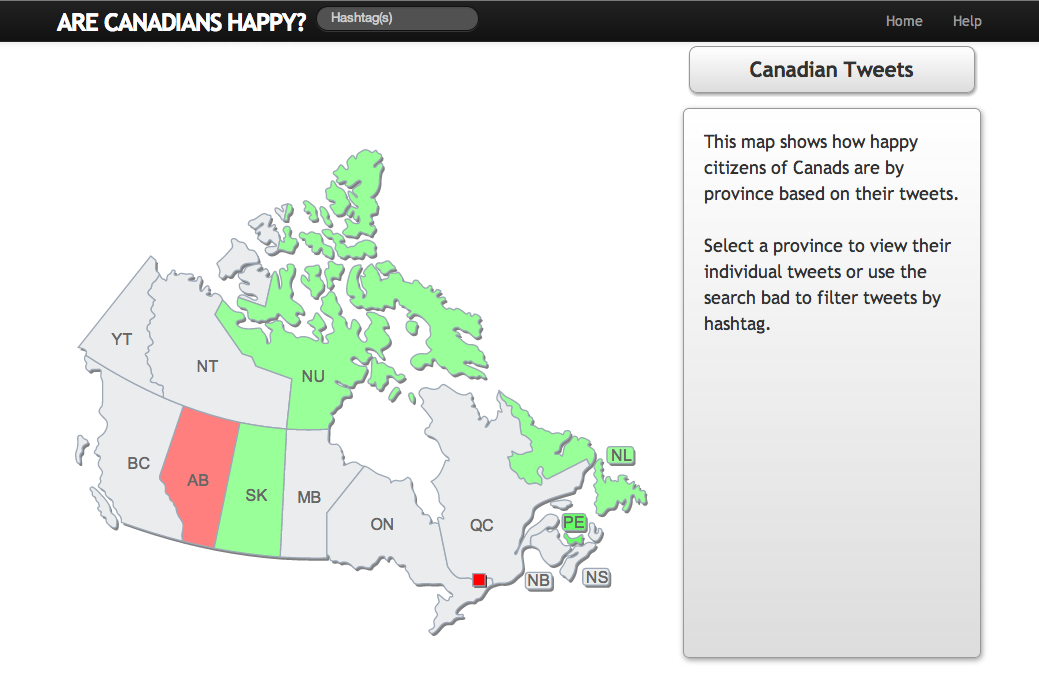
\includegraphics[width=0.9\textwidth]{images/website.png}
\caption{A screen shot of the Are Canadians Happy? website.\label{fig:website}}
\end{figure*}

\subsection{Collecting Tweets}

In order to collect Tweets from Twitter, a few choices has to be made in regards to the Twitter API. First,
the normal Twitter API is a REST API which allows the user to preform the typical REST requestions such as 
lookup and search. The problem with this technique is that for the purposes of ACH, we do not know what Tweets
we will be needing to find before hand, other that they are from Canada. So normally you would just do a
GET request for Tweets coming out of Canada, but unfortunately, Twitter does not allow for Tweet search
by location. This only leaves us with the option of using the Twitter Stream API. This API is slightly different
from the REST API because it does not issues static requests, but rather opens up a stream with parameters and
continually recieves new updates from Twitter as a random sample of current Tweets which fit the parameter 
criteria supplied by the user. In this case, our parameter criteria is that the Tweets come from Canada. The
only problem with this apporach is that Twitter only accepts latitude and longitude coordinate bounding 
boxes as locations. This being the case, I had to create a box around Canada, but unfortunately, Canada is
not square, so some United States Tweets are picked up from the stream and must be ignored in the final
analysis.

Once the Twitter stream data is being collected, it must be stored. For a storing option, I chose a PostgreSQL
database  in order to persistantly store Tweets. Between the collecting and storing of Tweets, Python scripts
were exclusively used to accomplish all of these actions. Python had mature plugin packages for both Twitter
and for connections to the PostgreSQL database so it was an easy choice and allowed for quicker development
than most other languages would allow. The only challenge with the Python sctips is that connections to the
database or the stream API can be lost over long periods of time. In order to overcome this challenge, monitoring
sciprts had to be setup on the server which the website resides to ensure that these Python scripts are always
running. This was the first instance of the crontab coming into use. The crontab on Linux machines allows for
jobs to be run periodically as set up by the owner. I made monitor scripts run every 5 minutes that checked
that the Python scipts were running and to restart them if they weren't.

The only other consideration for the collecting of Tweets is the storage time. Since I am now collectiong
around 100,000 Tweets per day, database storage must be considered. In order to avoid storing a massive
amount of Tweets, I set a limit of 48 hours for a Tweet's lifetime int he database. This ensures that any
sort of trends detected by ACH is only relevant to the newest Tweets. To enforce this decision, I created
another Python script to run every night at midnight (through the cron tab) which deletes the Tweets older
than 48 hours from the database. This final step completes the Tweet collection and storage implementation.

\subsection{Tweet Analysis}

In order to determine if Canadians are happy, I had to analyze every Tweet collected for topics and for
happiness or sentiment score. To do this, I used Python scripts again as a way to process the stream data
as it came in from Twitter. 

For every Tweet that came in, every word of the Tweet was seperated in order to analyze them on their own.
Each word was assigned a sentiment score as per the document handed out in this class for assignment 1
known as AFINN-111. This document has a variety of English language words with scores assigned to them
between -5 and +5. If a word is assigned a negative score then that means it has negative sentiment (sad, 
angry, etc.) and if it has a positive score it has a happy sentiment. As per the Tweets, each word is assigned
a score and the total score is for the Tweet is the aggregation of word scores within the Tweet. This final
score is also clamped between the values of -5 and +5 to avoid single Tweets scewing the results of
final analysis techniques. 

Aside from the total Tweet score, a goal of ACH is to analyzed Tweets by topics. With this being the case,
hashtags were also extracted from each Tweet in order to monitor what people are talking about to be able
to extract sentiments from topics across Canada later. A simple regex expression was used for this to
extract hashtag topics from the Tweets. These hashtag topics were also stored in the PostgreSQL database
along with the sentiment scores previously calculated.

\subsection{Visualization}

In order to provide a visualization to whether or not Canadians are happy, I chose to create a website
that utilized some quick prototyping technologies. I chose Ruby on Rails as the prime backbone of the ACH
website in order to create a quick infrastructure for the query style applicaton I needed. Ruby on rails
also allows for the use of external libraries to be quickly inserted and used along side the native Ruby
code. This being the case, I also added an HTML5 interactive map of Canada that I purchased from online
(maps of countries are usually not open source) to from the center peice of the application.

Now that I had a web framework in place and a map to use, I could simply query my database on the
home page load in order to find all Tweets from canada and aggregate them across provinces and their
scores in order to give a final result of each province in Canada for how happy they are. I will break
this process down into a few steps. First, in order to analyze the aggregation of sentiment scores
across provinces, I need some sort of aggregate function. The natural choice here was the use to the
avergae score per province. This works fairly well, except when a lot of tweets have scores of 1 or -1 
as the avergae very quickly becomes zero which makes for boring visualizaton. I played with the ideas of
mode and exlucing certain Tweets but this is a discussion for future work. Next I had to get these scores
from the Ruby backend to some Javascript front end. To do this I used the plugin known as ``gon'' which allows
the serialization of Ruby objects to JSON data. Once the data was in the frontend, I used from Javascript
in order to color the HTML5 map of Canada, per province, based on how happy or sad a province's Tweets
were. Red represented sad and green was happy. The darker the shade of the respective colors, the more
heavily the province leanded towards that emotion. 

% Map
\begin{figure}[tb!]
\centering
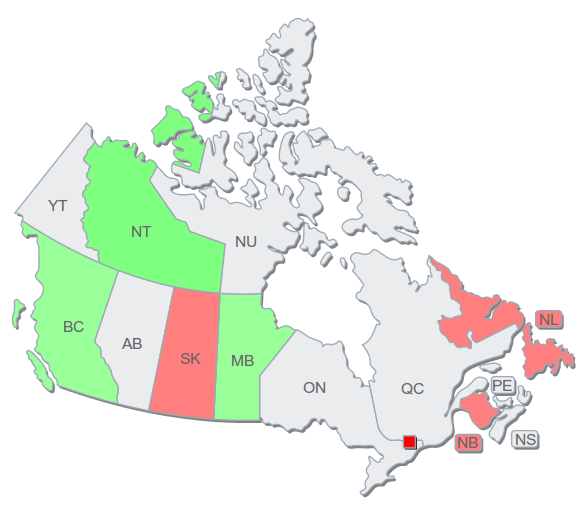
\includegraphics[width=0.5\textwidth]{images/map.png}
\caption{A screen shot of the Are Canadians Happy? website home view and map.\label{fig:map}}
\end{figure}

Aside from the map showing the aggregation of Tweet scores by specific colors, ACH also shows the latest
Tweets per province once they are clicked in the province stream. I show the last 10 Tweets of the province
and also color these in the same manor that the provinces are colored.

% Map
\begin{figure}[tb!]
\centering
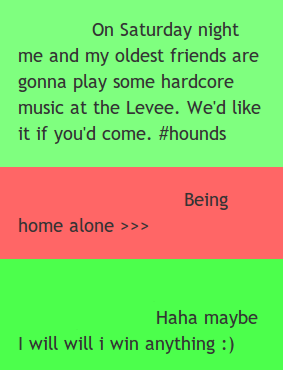
\includegraphics[width=0.5\textwidth]{images/stream.png}
\caption{A screen shot of the Are Canadians Happy? Twitter stream.\label{fig:stream}}
\end{figure}

Not only can a user of this website determine the overall nature of Canadians and their sentiment
levels inside of Twitter, but they can also use the website to check specific hashtag topics and how
Canadians feel about them. In order to do this, a user can use the search bar found at the top of the
website and search for a specific hashtag. What this does, is filter all Tweets to those which contain
the speicific hashtag and then performs the same aggregation and coloring of provinces based on those
filtered Tweets. This allows users to explore more deeply in Canada the trends of sentiment coming from
this nation.

% Map
\begin{figure}[tb!]
\centering

\includegraphics[width=0.5\textwidth]{images/search.png}
\caption{A screen shot of the Are Canadians Happy search bar.\label{fig:search}}
\end{figure}

The website also has several static pages in order to help the user understand how to use the website, how
it works, and a form to submit ideas for future improvements of the website.

\section{Future Work}
\label{sec:fw}

For future work, I hope to implement more options for analysis to the end user. One of the major
analysis workings I hope to provide is the ability to choose how sentiment score will be aggregated
across Tweets for a province. Right now, as was mentioned earlier, a simple average is taken, however
this is not always the best choice. In some cases, mode may be a more appropriate choice, or there
might be a case where outliers are more important than the avergae so some options to end users to
provide these types of analysis should be provided.

In terms of natural language processing, not much is being done right now in the current application.
In terms of detecting topics being discusses in Canada, so far only hashtags are being used. This is extremely
limited in what else can be done. These exists techniques that allow for key words and trending topics
to be identified. I plan to use these techniques in the future to supplement and compliment the structured
hashtags that come out of Twitter so that users of this site can identify trends that may not be explicity
mentioned inside of Tweets.

Another processing technique I would like to use for future analysis is keyword paring to topics. For instance
if people use the word ``mad'' everytime they use the hashtags \#GOC, we can identify a trend of Canadians
being mad at the government of Canada. This allows for slightly deeper analysis of the sentiments coming
out of Canada regarding some Tweets.

Finally, as a long down the road plan, I hope to take these same techniques for data collection and visualization
and apply them to more unstructured data from around the web and not just Twitter. Blogs, forums and other social 
media outlets on the web contain an extensive amount of unstructured data that is ripe for the picking in terms
of big data analysis and so far it has gone largely ununtilized. By gathering and analyzing this data, I hope
to provide stronger results on my types of sentiment analysis moving into the future.

\section{Conclusions}
\label{sec:conc}

This paper has walked through the creation and implementation of the website ``Are Canadians Happy?''.
I have shown how through the use of the Twitter Stream API, and a few other basic data storage and
web technologies, we can create tools which can perform deep analysis on natural unstructured data that
is avaliable throughout the web. Moving forward, I do not only hope to improve my website by the better
analysis of Twitter and natural language processing, but I also hope to open the ideas of this
paper to futher unstructured data on the web from forums and other social media forms.

I hope to release ``Are Canadians Happy?'' to a public webserver sometime before the end of 2013. Once
this occurs, the public will be able to access all workings found in this paper in a clean and polished 
format website.


% End of the paper
\end{document}
